

\section{Experiment motivation}
\clearpage
\section{Experiment setup}
\clearpage
\section{Environment}
\clearpage
\section{Roborobo overview}
	\subsection{Agent observers}
	\subsection{Agent controllers}
	\subsection{World observers}
\clearpage
\section{Roborobo modifications}
	\subsection{Robot Groups}
	\subsubsection{Movement}
	\subsubsection{Collisions}
	\subsubsection{Disconnecting}

	\subsection{Connection mechanism}
		\subsubsection{Connection validation}
	\subsection{Local communication}
		\subsubsection{Message aggregation, message lattice}
	\subsection{Predators}
		\subsubsection{Search strategy}
		\subsubsection{Hunting strategy}
	\subsection{Energy drain}
		\subsubsection{Passive}
		\subsubsection{Active}
\clearpage
\section{CTRNN}
For this project, an artificial neural network that has gained a lot a popularity in regards to robotics known as Continuous-Time Recurrent Neural Network (CTRNN) was implemented. 
The CTRNN was researched and developed by Randall Beer and adds two new properties to the standard artificial neural network. 
The properties that are introduced in CTRNN is a time constant and a gain.

As most neural networks, the simple integration of the inputs from all neighbouring neurons are added giving us the first standard equation for neural networks:

\begin{equation}
	s_i = \sum_{j=1}^{n}o_{j}w_{i,j}+I_i
\end{equation}
\\
Here, $o_j$ represents the output(after activation) of neuron $j$, $w_{i,j}$ is the weight from neuron $j$ to neuron $i$ and $I_i$ is the sum of all the external inputs to node $i$.

\begin{equation}
\frac{dy_i}{dt} = \frac{1}{\tau_i}[-y_i + s_i + \theta_i]
\end{equation}
\\
In order to preserve the previous state of the ANN, the internal state is stored. 
$y_i$ denotes the internal state of neuron $i$.
To derive the next internal state, Beer computes $\frac{dy_i}{dt}$ as a combination of the next inputs and the current internal state of the node, where a time constant $\tau_i$ decides rate of drain. 
$\theta_i$ is a term added for neuron specific bias, but is only added here for mathematical soundness as it was simply added as a bias node during implementation and hence incorporated in $s_i$.
The time constant $\tau_i$ is what gives CTRNNs the ability to produce rich functionality and convincingly sophisticated cognition.
If $\tau_i$ has a low value then we will have a high degree of drain and hence having the next state being dominated by its new input.
However, if $\tau_i$ has a high value, then we have a higher degree of memory because it will be dominated by its previous state.

\begin{equation}
o_i = \frac{1}{1 + e^{-g_{i}y_{i}}}
\end{equation}
\\
To convert the internal state to an output $o_i$, Beer typically uses sigmoidal activation function.
This is typical in other neural networks as well, but Beer also employs a gain term $g_i$, to influence the activation of the neuron.
\\
\begin{figure}[H]
	\centering
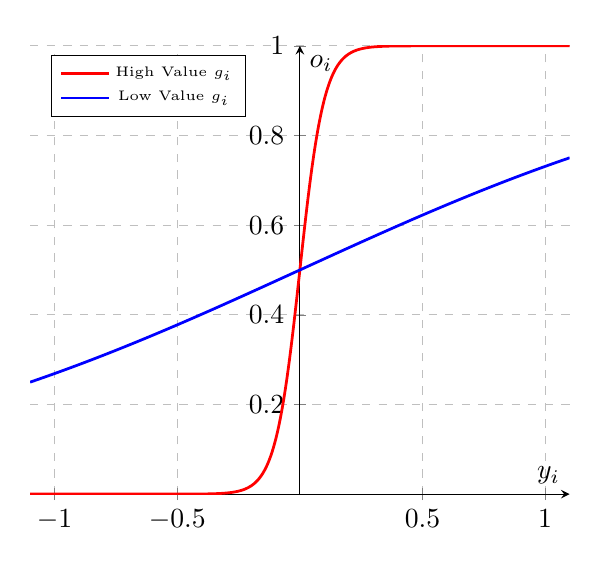
\begin{tikzpicture}
\begin{axis}[
	axis lines = center,
    xlabel = $y_i$,
    ylabel = {$o_i$},
    ymajorgrids=true,
    xmajorgrids=true,
    grid style=dashed,
    legend style={at={(0.22, 0.98)},anchor=north, font=\tiny}
]
%Below the red parabola is defined
\addplot [
    domain=-1.1:1.1, 
    samples=500, 
    color=red,
    line width=1pt,
]
{1/(1+e^(-20*x)};
\addlegendentry{High Value $g_i$}
%Here the blue parabloa is defined
\addplot [
    domain=-1.1:1.1, 
    samples=100, 
    color=blue,
	line width=1pt,
]
{1/(1+e^(-1*x)};
\addlegendentry{Low Value $g_i$}
 
\end{axis}
\end{tikzpicture}
	\caption{The difference in the activation function with respect to $y_i$ based on a low and high value of $g_i$}
	\label{CTRNN-gGraph}
\end{figure}

As seen in figure \ref{CTRNN-gGraph}, the value of the gain parameter can influence the activation function in such a way that it can be a smooth, almost linear, function or it can take on the behaviour of an activation function resembling a switch.
Having the ability to change the activation function on a neuron to neuron basis, is the second reason(the first being time constants) CTRNNs can give rise to complex and rich behaviour.



	\subsection{Drain}
	\subsection{Activation function}
	\subsection{Topologies}
		\subsubsection{Dense}
		\subsubsection{Sparse}
\clearpage
\section{Evolutionary algorithm}
	\subsection{Genotype}
	\subsection{Initialization}
	\subsection{Mutation operators}
		\subsubsection{Random}
		\subsubsection{Incremental}
	\subsection{Selection mechanism}
\clearpage
\section{Data gathering}
	\section{Loggers}
	\section{Analysis}
\clearpage
\subsection{Extras/Appendix?}
	\subsection{Parallelization}
	\subsection{Python graph tool}
	\subsection{System configuration}
\clearpage
	